\documentclass[a4paper]{article}
\usepackage{amsmath} % Define various maths environments
\usepackage{amssymb} % Define various maths symbols
\usepackage{geometry} % Adjust the margin, paper size, and etc.
\geometry{left=2.5cm,right=2.5cm,top=3cm,bottom=3cm}
\usepackage{enumerate} % Provide different style of lists
\usepackage{graphicx}
\usepackage{float}
\usepackage{listings} 

\title{—————————————————————————\\ \sc{UM-SJTU Joint Institute}}
\author{\sc{Data Structures and Algorithms}}
\date{\sc{(Ve281)}\\——————————————————————————————}

\begin{document}
\maketitle
\vspace{5cm}
\centerline{\Large{\sc{Lab 05 Report}}}
\vspace{9cm}
\begin{tabular}{lll}
\qquad \qquad Name: Sun Yiwen&ID: 517370910213\\
\qquad \qquad Date: 13 November 2019
\end{tabular}

\newpage
\section{Runtime Analysis}
\noindent
\par
I tested the three heap implementations with input size $n=10\times10,20\times20,50\times50,100\times100,200\times200,500\times500$. The data are shown in the following table and the runtime analysis result is shown in Figure 1. In Figure 2, runtime of input size $n=250000$ is deleted in order to demonstrate the runtime difference between these three heap implementations (when the input size is small) more clearly. Compared with binary heap and Fibonacci heap, unsorted heap is significantly less efficient. This corresponds with the theoretical finding that Fibanacci heap and binary heap have faster time complexity than unsorted heap.

\begin{figure}[htbp]
\centering
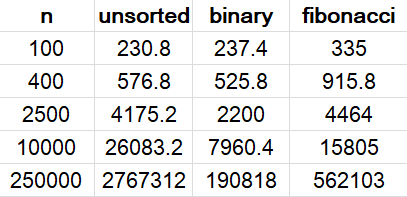
\includegraphics[scale=0.7]{p3new.png}
\end{figure}

\begin{figure}[htbp]
\centering
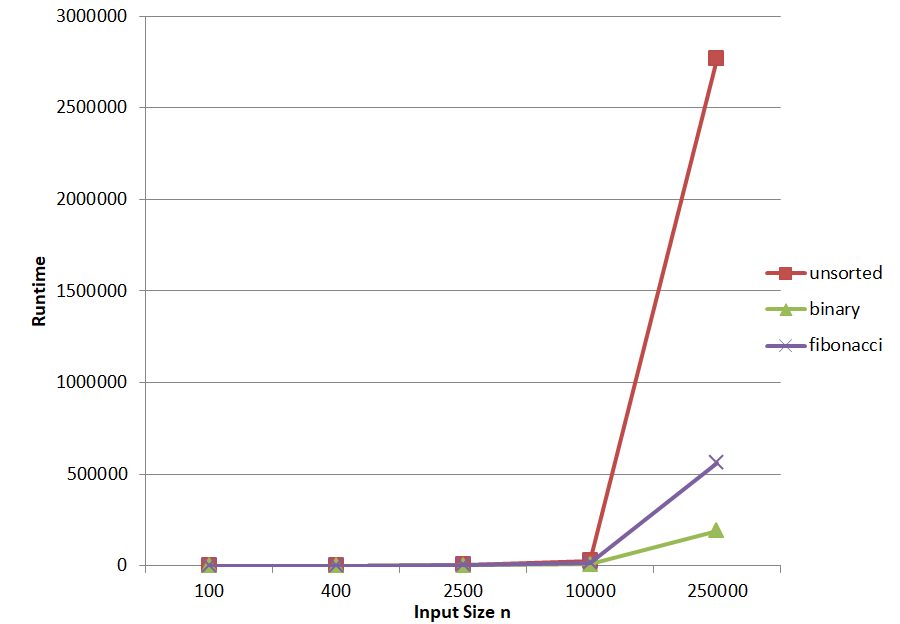
\includegraphics[scale=0.5]{p1new.png}
\caption{Plot of runtime vs. input size n of the three heap implementations. ($n_{max}=250000$)}
\end{figure}
\begin{figure}[htbp]
\centering
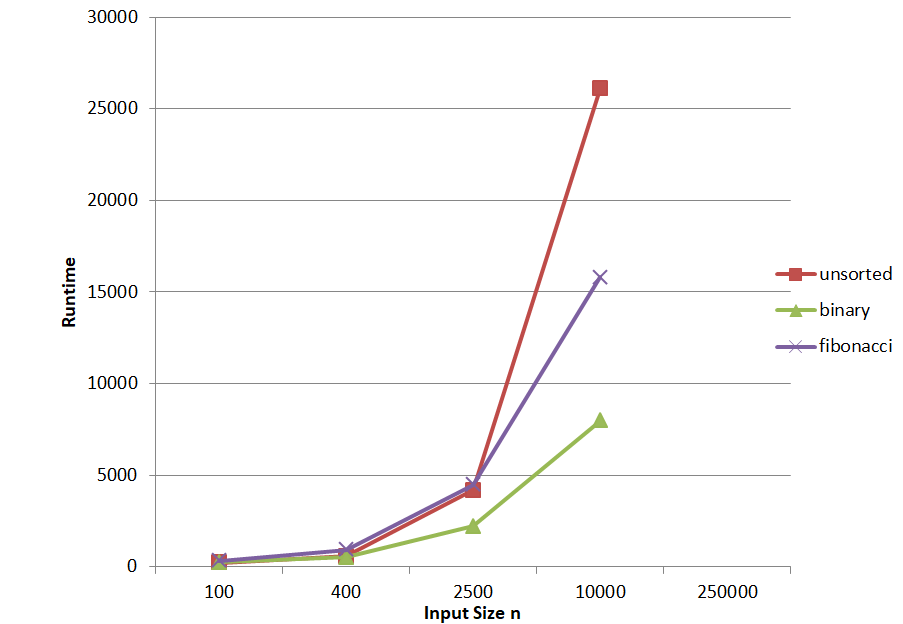
\includegraphics[scale=0.5]{p2new.png}
\caption{Plot of runtime vs. input size n of the three heap implementations. ($n_{max}=10000$)}
\end{figure}

\section{Theoretical Time Complexity}
\noindent
\par
As shown in Figure 3, the theoretical time complexity of enqueue operation for binary heap is O(log n) while the time complexity of enqueue operation for Fibonacci heap is O(1). However, as we look at the previous section "Runtime Analysis", we found that the runtime of binary heap is faster than Fibonacci heap. This is probably because the constant time used in Fibonacci heap implementation is much longer than that in binary heap and it makes the total runtime longer.

\begin{figure}[htbp]
\centering
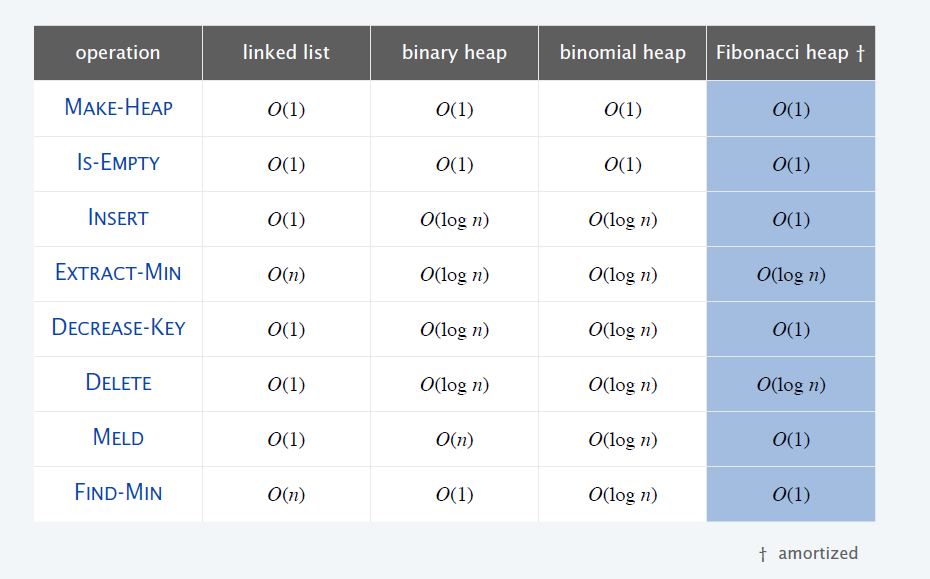
\includegraphics[scale=0.8]{p4.png}
\caption{Priority queues performance cost summary}
\end{figure}


\section{Code}
\subsection{priority$\_{}$queue.h}
\begin{lstlisting}[language=C++] 
#ifndef PRIORITY_QUEUE_H
#define PRIORITY_QUEUE_H

#include <functional>
#include <vector>

// OVERVIEW: A simple interface that implements a generic heap.
//           Runtime specifications assume constant time comparison and
//           copying. TYPE is the type of the elements stored in the priority
//           queue. COMP is a functor, which returns the comparison result of
//           two elements of the type TYPE. See test_heap.cpp for more details
//           on functor.
template<typename TYPE, typename COMP = std::less<TYPE> >
class priority_queue {
public:
  typedef unsigned size_type;

  virtual ~priority_queue() {}

  // EFFECTS: Add a new element to the heap.
  // MODIFIES: this
  // RUNTIME: O(n) - some implementations *must* have tighter bounds (see
  //          specialized headers).
  virtual void enqueue(const TYPE &val) = 0;

  // EFFECTS: Remove and return the smallest element from the heap.
  // REQUIRES: The heap is not empty.
  //           Note: We will not run tests on your code that would require it
  //           to dequeue an element when the heap is empty.
  // MODIFIES: this
  // RUNTIME: O(n) - some implementations *must* have tighter bounds (see
  //          specialized headers).
  virtual TYPE dequeue_min() = 0;

  // EFFECTS: Return the smallest element of the heap.
  // REQUIRES: The heap is not empty.
  // RUNTIME: O(n) - some implementations *must* have tighter bounds (see
  //          specialized headers).
  virtual const TYPE &get_min() const = 0;

  // EFFECTS: Get the number of elements in the heap.
  // RUNTIME: O(1)
  virtual size_type size() const = 0;

  // EFFECTS: Return true if the heap is empty.
  // RUNTIME: O(1)
  virtual bool empty() const = 0;

};

#endif //PRIORITY_QUEUE_H

\end{lstlisting}

\subsection{unsorted$\_{}$heap.h}
\begin{lstlisting}[language=C++]
#ifndef UNSORTED_HEAP_H
#define UNSORTED_HEAP_H

#include <algorithm>
#include "priority_queue.h"

// OVERVIEW: A specialized version of the 'heap' ADT that is implemented with
//           an underlying unordered array-based container. Every time a min
//           is required, a linear search is performed.
template<typename TYPE, typename COMP = std::less<TYPE> >
class unsorted_heap: public priority_queue<TYPE, COMP> {
public:
  typedef unsigned size_type;

  // EFFECTS: Construct an empty heap with an optional comparison functor.
  //          See test_heap.cpp for more details on functor.
  // MODIFIES: this
  // RUNTIME: O(1)
  unsorted_heap(COMP comp = COMP());

  // EFFECTS: Add a new element to the heap.
  // MODIFIES: this
  // RUNTIME: O(1)
  virtual void enqueue(const TYPE &val);

  // EFFECTS: Remove and return the smallest element from the heap.
  // REQUIRES: The heap is not empty.
  // MODIFIES: this
  // RUNTIME: O(n)
  virtual TYPE dequeue_min();

  // EFFECTS: Return the smallest element of the heap.
  // REQUIRES: The heap is not empty.
  // RUNTIME: O(n)
  virtual const TYPE &get_min() const;

  // EFFECTS: Get the number of elements in the heap.
  // RUNTIME: O(1)
  virtual size_type size() const;

  // EFFECTS: Return true if the heap is empty.
  // RUNTIME: O(1)
  virtual bool empty() const;

private:
  std::vector<TYPE> data;
  COMP compare;
};

template<typename TYPE, typename COMP>
unsorted_heap<TYPE, COMP> :: unsorted_heap(COMP comp) {
    compare = comp;
}

template<typename TYPE, typename COMP>
void unsorted_heap<TYPE, COMP> :: enqueue(const TYPE &val) {
	this->data.push_back(val);
}

template<typename TYPE, typename COMP>
TYPE unsorted_heap<TYPE, COMP> :: dequeue_min() {
	unsigned int i, min_num;
	static TYPE min;
	min_num = 0;
	min = this->data[0];
	for (i = 1; i < this->size(); i++) {
		if (compare(this->data[i], min)) {
			min = this->data[i];
			min_num = i;
		}
	}
	this->data[min_num] = this->data[i - 1];
	this->data.pop_back();
	return min;
}

template<typename TYPE, typename COMP>
const TYPE &unsorted_heap<TYPE, COMP> :: get_min() const {
	unsigned int i;
	static TYPE min;
	min = this->data[0];
	for (i = 1; i < this->size(); i++) {
		if (compare(this->data[i], min)) min = this->data[i];
	}
	return min;
}

template<typename TYPE, typename COMP>
bool unsorted_heap<TYPE, COMP> :: empty() const {
	return this->data.empty();
}

template<typename TYPE, typename COMP>
unsigned unsorted_heap<TYPE, COMP> :: size() const { 
	return this->data.size();
}

#endif //UNSORTED_HEAP_H
\end{lstlisting}

\subsection{binary$\_{}$heap.h}
\begin{lstlisting}[language=C++]
#ifndef BINARY_HEAP_H
#define BINARY_HEAP_H

#include <algorithm>
#include "priority_queue.h"

// OVERVIEW: A specialized version of the 'heap' ADT implemented as a binary
//           heap.
template<typename TYPE, typename COMP = std::less<TYPE> >
class binary_heap: public priority_queue<TYPE, COMP> {
public:
  typedef unsigned size_type;

  // EFFECTS: Construct an empty heap with an optional comparison functor.
  //          See test_heap.cpp for more details on functor.
  // MODIFIES: this
  // RUNTIME: O(1)
  binary_heap(COMP comp = COMP());

  // EFFECTS: Add a new element to the heap.
  // MODIFIES: this
  // RUNTIME: O(log(n))
  virtual void enqueue(const TYPE &val);

  // EFFECTS: Remove and return the smallest element from the heap.
  // REQUIRES: The heap is not empty.
  // MODIFIES: this
  // RUNTIME: O(log(n))
  virtual TYPE dequeue_min();

  // EFFECTS: Return the smallest element of the heap.
  // REQUIRES: The heap is not empty.
  // RUNTIME: O(1)
  virtual const TYPE &get_min() const;

  // EFFECTS: Get the number of elements in the heap.
  // RUNTIME: O(1)
  virtual size_type size() const;

  // EFFECTS: Return true if the heap is empty.
  // RUNTIME: O(1)
  virtual bool empty() const;

private:
  std::vector<TYPE> data;
  COMP compare;

private:
	void swap(TYPE& a, TYPE& b);
	void perculateUp(int id);
	void perculateDown(int id);
};

template<typename TYPE, typename COMP>
void binary_heap<TYPE, COMP>::swap(TYPE& a, TYPE& b) {
	TYPE temp;
	temp = a;
	a = b;
	b = temp;
}

template<typename TYPE, typename COMP>
void binary_heap<TYPE, COMP>::perculateUp(int id) {
	while (id > 0 && compare(this->data[id], this->data[(id + 1) / 2 - 1])) {
		swap(this->data[(id + 1) / 2 - 1], this->data[id]);
		id = (id + 1) / 2 - 1;
	}
}

template<typename TYPE, typename COMP>
void binary_heap<TYPE, COMP>::perculateDown(int id) {
	unsigned int j;
	for (j = 2 * (id + 1) - 1; j < this->data.size(); j = 2 * (id + 1) - 1) {
		if (j < this->data.size() - 1 
		&& compare(this->data[j + 1], this->data[j])) j++;
		if (!compare(this->data[j], this->data[id])) break;
		swap(this->data[id], this->data[j]);
		id = j;
	}
}

template<typename TYPE, typename COMP>
binary_heap<TYPE, COMP> :: binary_heap(COMP comp) {
    compare = comp;
}

template<typename TYPE, typename COMP>
void binary_heap<TYPE, COMP> :: enqueue(const TYPE &val) {
	this->data.push_back(val);
	perculateUp(this->data.size() - 1);
}

template<typename TYPE, typename COMP>
TYPE binary_heap<TYPE, COMP> :: dequeue_min() {
	TYPE min;
	min = this->data[0];
	swap(this->data[0], this->data[this->data.size() - 1]);
	this->data.pop_back();
	perculateDown(0);
	return min;
}

template<typename TYPE, typename COMP>
const TYPE &binary_heap<TYPE, COMP> :: get_min() const {
	return this->data[0];
}

template<typename TYPE, typename COMP>
bool binary_heap<TYPE, COMP> :: empty() const {
	return this->data.empty();
}

template<typename TYPE, typename COMP>
unsigned binary_heap<TYPE, COMP> :: size() const { 
	return this->data.size();
}

#endif //BINARY_HEAP_H
\end{lstlisting}

\subsection{fib$\_{}$heap.h}
\begin{lstlisting}[language=C++]
#ifndef FIB_HEAP_H
#define FIB_HEAP_H

#include <algorithm>
#include <cmath>
#include "priority_queue.h"

// OVERVIEW: A specialized version of the 'heap' ADT implemented as a 
//           Fibonacci heap.
template<typename TYPE, typename COMP = std::less<TYPE> >
class fib_heap : public priority_queue<TYPE, COMP> {
public:
	typedef unsigned size_type;

	// EFFECTS: Construct an empty heap with an optional comparison functor.
	//          See test_heap.cpp for more details on functor.
	// MODIFIES: this
	// RUNTIME: O(1)
	fib_heap(COMP comp = COMP());

	// EFFECTS: Deconstruct the heap with no memory leak.
	// MODIFIES: this
	// RUNTIME: O(n)
	~fib_heap();

	// EFFECTS: Add a new element to the heap.
	// MODIFIES: this
	// RUNTIME: O(1)
	virtual void enqueue(const TYPE& val);

	// EFFECTS: Remove and return the smallest element from the heap.
	// REQUIRES: The heap is not empty.
	// MODIFIES: this
	// RUNTIME: Amortized O(log(n))
	virtual TYPE dequeue_min();

	// EFFECTS: Return the smallest element of the heap.
	// REQUIRES: The heap is not empty.
	// RUNTIME: O(1)
	virtual const TYPE& get_min() const;

	// EFFECTS: Get the number of elements in the heap.
	// RUNTIME: O(1)
	virtual size_type size() const;

	// EFFECTS: Return true if the heap is empty.
	// RUNTIME: O(1)
	virtual bool empty() const;

private:
	// Note: compare is a functor object
	COMP compare;

private:
	struct node {
		TYPE key;
		node* parent;
		node* child;
		node* left;
		node* right;
		int rank;
	};
	int num;
	node* MinNode;

	void destruct();
	void Consolidate();
	void Link(node* y, node* x);
};

template<typename TYPE, typename COMP>
void fib_heap<TYPE, COMP>::Link(node* y, node* x) {
	y->left->right = y->right;
	y->right->left = y->left;
	y->parent = x;
	if (x->child != NULL) {
		y->left = x->child;
		y->right = x->child->right;
		x->child->right->left = y;
		x->child->right = y;
	}
	else {
		y->left = y;
		y->right = y;
		x->child = y;
	}
	x->rank++;
}

template<typename TYPE, typename COMP>
void fib_heap<TYPE, COMP>::Consolidate() {
	int size = floor(log(this->num) / log(1.618)) + 1;
	node* A[size];
	node* start = this->MinNode;
	A[this->MinNode->rank] = this->MinNode;
	node* next = this->MinNode->right;
	int num_root = 1;
	for (int i = 0; i < size; i++) A[i] = NULL;
	while (next != start) {
		num_root++;
		next = next->right;
	}
	for (int i = 0; i < num_root; i++) {
		node* x = next;
		next = x->right;
		int d = x->rank;
		while (A[d] != NULL) {
			node* y = A[d];
			if (compare(y->key, x->key)) {
				node* temp = y;
				y = x;
				x = temp;
			}
			Link(y, x);
			A[d] = NULL;
			d++;
		}
		A[d] = x;
	}
	this->MinNode = NULL;
	for (int i = 0; i < size; i++) {
		if (A[i] != NULL) {
			if (this->MinNode == NULL) {
				this->MinNode = A[i];
				this->MinNode->left = this->MinNode;
				this->MinNode->right = this->MinNode;
				this->MinNode->parent = NULL;
			}
			else {
				A[i]->left = this->MinNode;
				A[i]->right = this->MinNode->right;
				A[i]->parent = NULL;
				this->MinNode->right->left = A[i];
				this->MinNode->right = A[i];
				if (compare(A[i]->key, this->MinNode->key))
				 this->MinNode = A[i];
			}
		}
	}
}


template<typename TYPE, typename COMP>
fib_heap<TYPE, COMP> ::fib_heap(COMP comp) {
	compare = comp;
	num = 0;
	MinNode = NULL;
}

template<typename TYPE, typename COMP>
void fib_heap<TYPE, COMP> ::enqueue(const TYPE& val) {
	node* x = new node;
	x->key = val;
	x->parent = NULL;
	x->child = NULL;
	x->rank = 0;

	if (this->MinNode == NULL) {
		x->left = x;
		x->right = x;
		this->MinNode = x;
	}
	else {
		x->left = this->MinNode;
		x->right = this->MinNode->right;
		this->MinNode->right->left = x;
		this->MinNode->right = x;
		if (compare(x->key, this->MinNode->key)) this->MinNode = x;
	}
	this->num++;
}

template<typename TYPE, typename COMP>
TYPE fib_heap<TYPE, COMP> ::dequeue_min() {
	TYPE min;
	min = this->MinNode->key;
	if (this->MinNode->child != NULL) {
		while (this->MinNode->child->right != this->MinNode->child) {
			node* temp1;
			temp1 = this->MinNode->child->right;
			this->MinNode->child->right->right->left 
			= this->MinNode->child;
			this->MinNode->child->right 
			= this->MinNode->child->right->right;
			temp1->left = this->MinNode;
			temp1->right = this->MinNode->right;
			temp1->parent = NULL;
			this->MinNode->right->left = temp1;
			this->MinNode->right = temp1;
		}
		node* temp2;
		temp2 = this->MinNode->child;
		temp2->left = this->MinNode;
		temp2->right = this->MinNode->right;
		temp2->parent = NULL;
		this->MinNode->right->left = temp2;
		this->MinNode->right = temp2;
		this->MinNode->child = NULL;
	}
	node* temp3 = this->MinNode;
	this->MinNode->left->right = this->MinNode->right;
	this->MinNode->right->left = this->MinNode->left;
	this->num--;
	if (this->num == 0) this->MinNode = NULL;
	else {
		node* newmin = this->MinNode->right;
		node* stay = newmin;
		node* find = newmin->right;
		while (find != stay) {
			if (compare(find->key, newmin->key)) newmin = find;
			find = find->right;
		}
		this->MinNode = newmin;
		Consolidate();
	}
	delete temp3;
	return min;
}


template<typename TYPE, typename COMP>
const TYPE& fib_heap<TYPE, COMP> ::get_min() const {
	return this->MinNode->key;
}

template<typename TYPE, typename COMP>
bool fib_heap<TYPE, COMP> ::empty() const {
	return (this->MinNode == NULL);
}

template<typename TYPE, typename COMP>
unsigned fib_heap<TYPE, COMP> ::size() const {
	return this->num;
}

template<typename TYPE, typename COMP>
void fib_heap<TYPE, COMP> ::destruct() {
	if (this->MinNode == NULL) return;
	bool hasRight = false, hasChild = false;
	node* current = this->MinNode;
	if (current->right != current) hasRight = true;
	if (current->child != NULL) hasChild = true;
	if (current->parent != NULL && current->parent->child == current) {
		if (current->right != current) {
			current->parent->child = current->right;
		}
		else current->parent->child = NULL;
	}
	if (current->right != current) {
		current->right->left = current->left;
		current->left->right = current->right;
	}
	if (hasRight) {
		this->MinNode = current->right;
		destruct();
	}
	if (hasChild) {
		this->MinNode = current->child;
		destruct();
	}
	delete current;
	return;
}

template<typename TYPE, typename COMP>
fib_heap<TYPE, COMP> ::~fib_heap() {
	destruct();
}

#endif //FIB_HEAP_H
\end{lstlisting}

\subsection{main.cpp}
\begin{lstlisting}[language=C++]
#include <iostream>
#include <fstream>
#include <getopt.h>
#include <ctime>
#include "unsorted_heap.h"
#include "binary_heap.h"
#include "fib_heap.h"
using namespace std;

struct point {
	int location_x, location_y;
	unsigned int cellweight;
	unsigned int pathcost;
	bool Reached;
	point* predecessor;
};

struct compare_t
{
	bool operator()(point* a, point* b) const
	{
		if (a->pathcost == b->pathcost) {
			if (a->location_x == b->location_x) 
			return a->location_y < b->location_y;
			else return a->location_x < b->location_x;
		}
		else return a->pathcost < b->pathcost;
	}
};

void trace_back_path(point *current) {
	if (current->predecessor == NULL) 
	cout << "(" << current->location_x << ", " << current->location_y 
	<< ")" << endl;
	else {
		trace_back_path(current->predecessor);
		cout << "(" << current->location_x << ", " 
		<< current->location_y << ")" << endl;
	}
}

void print(point& start, point& end) {
	cout << "The shortest path from (" << start.location_x << ", " 
	<< start.location_y << ") to (" << end.location_x 
	<< ", " << end.location_y << ") is " << end.pathcost 
	<< "." << endl;
	cout << "Path:" << endl;
	point *end_p = &end;
	trace_back_path(end_p);
}

void findPath(priority_queue<point*, compare_t>* PQ, bool verbose) {
	int i, j, step = 0;
	int width, height, start_x, start_y, end_x, end_y;

	cin >> width >> height >> start_x >> start_y >> end_x >> end_y;
	point** W = new point*[height];
	for (i = 0; i < height; i++) {
		W[i] = new point[width];
		for (j = 0; j < width; j++) {
			cin >> W[i][j].cellweight;
			W[i][j].location_y = i;
			W[i][j].location_x = j;
			W[i][j].pathcost = 0;
			W[i][j].Reached = false;
			W[i][j].predecessor = NULL;
		}
	}
	W[start_y][start_x].pathcost = W[start_y][start_x].cellweight;
	W[start_y][start_x].Reached = true;
	PQ->enqueue(&W[start_y][start_x]);
	while (!PQ->empty()) {
		if (verbose) cout << "Step " << step << endl;
		step++;
		point* C = PQ->dequeue_min();
		if (verbose) cout << "Choose cell (" << C->location_x 
		<< ", " << C->location_y << ") with accumulated length " 
		<< C->pathcost << "." << endl;
		if (C->location_x + 1 < width 
		&& (!W[C->location_y][C->location_x + 1].Reached)) {
			point* N1 = &W[C->location_y][C->location_x + 1];
			N1->pathcost = C->pathcost + N1->cellweight;
			N1->Reached = true;
			N1->predecessor = C;
			if (N1->location_y == end_y && N1->location_x == end_x) {
				if (verbose) 
				cout << "Cell (" << N1->location_x << ", " 
				<< N1->location_y << ") with accumulated length " 
				<< N1->pathcost << " is the ending point." << endl;
				cout << "The shortest path from (" 
				<< W[start_y][start_x].location_x << ", " 
				<< W[start_y][start_x].location_y << ") to (" 
				<< N1->location_x << ", " << N1->location_y << ") is " 
				<< N1->pathcost << "." << endl;
				cout << "Path:" << endl;
				trace_back_path(N1);
				return;
			}
			else if (verbose) {
				cout << "Cell (" << N1->location_x << ", " 
				<< N1->location_y << ") with accumulated length " 
				<< N1->pathcost << " is added into the queue." << endl;
				PQ->enqueue(N1);
			}
			else PQ->enqueue(N1);
		}
		if (C->location_y + 1 < height 
		&& (!W[C->location_y + 1][C->location_x].Reached)) {
			point* N2 = &W[C->location_y + 1][C->location_x];
			N2->pathcost = C->pathcost + N2->cellweight;
			N2->Reached = true;
			N2->predecessor = C;
			if (N2->location_y == end_y && N2->location_x == end_x) {
				if (verbose) cout << "Cell (" << N2->location_x 
				<< ", " << N2->location_y 
				<< ") with accumulated length " 
				<< N2->pathcost << " is the ending point." << endl;
				cout << "The shortest path from (" 
				<< W[start_y][start_x].location_x 
				<< ", " << W[start_y][start_x].location_y 
				<< ") to (" 
				<< N2->location_x << ", " 
				<< N2->location_y << ") is " << N2->pathcost 
				<< "." << endl;
				cout << "Path:" << endl;
				trace_back_path(N2);
				return;
			}
			else if (verbose) {
				cout << "Cell (" << N2->location_x 
				<< ", " << N2->location_y 
				<< ") with accumulated length " 
				<< N2->pathcost << " is added into the queue." 
				<< endl;
				PQ->enqueue(N2);
			}
			else PQ->enqueue(N2);
		}
		if (C->location_x > 0 
		&& (!W[C->location_y][C->location_x - 1].Reached)) {
			point* N3 = &W[C->location_y][C->location_x - 1];
			N3->pathcost = C->pathcost + N3->cellweight;
			N3->Reached = true;
			N3->predecessor = C;
			if (N3->location_y == end_y && N3->location_x == end_x) {
				if (verbose) cout << "Cell (" 
				<< N3->location_x << ", " << N3->location_y 
				<< ") with accumulated length " 
				<< N3->pathcost << " is the ending point." 
				<< endl;
				cout << "The shortest path from (" 
				<< W[start_y][start_x].location_x 
				<< ", " << W[start_y][start_x].location_y 
				<< ") to (" << N3->location_x << ", " 
				<< N3->location_y << ") is " << N3->pathcost 
				<< "." << endl;
				cout << "Path:" << endl;
				trace_back_path(N3);
				return;
			}
			else if (verbose) {
				cout << "Cell (" << N3->location_x 
				<< ", " << N3->location_y 
				<< ") with accumulated length " 
				<< N3->pathcost << " is added into the queue." 
				<< endl;
				PQ->enqueue(N3);
			}
			else PQ->enqueue(N3);
		}
		if (C->location_y > 0 
		&& (!W[C->location_y - 1][C->location_x].Reached)) {
			point* N4 = &W[C->location_y - 1][C->location_x];
			N4->pathcost = C->pathcost + N4->cellweight;
			N4->Reached = true;
			N4->predecessor = C;
			if (N4->location_y == end_y && N4->location_x == end_x) {
				if (verbose) cout << "Cell (" << N4->location_x 
				<< ", " << N4->location_y 
				<< ") with accumulated length "
				 << N4->pathcost << " is the ending point." << endl;
				cout << "The shortest path from (" 
				<< W[start_y][start_x].location_x 
				<< ", " << W[start_y][start_x].location_y << ") to (" 
				<< N4->location_x << ", " << N4->location_y 
				<< ") is " << N4->pathcost << "." << endl;
				cout << "Path:" << endl;
				trace_back_path(N4);
				return;
			}
			else if (verbose) {
				cout << "Cell (" << N4->location_x << ", " 
				<< N4->location_y << ") with accumulated length " 
				<< N4->pathcost << " is added into the queue." << endl;
				PQ->enqueue(N4);
			}
			else PQ->enqueue(N4);
		}
	}
}

void create_unsorted(bool verbose) {
	priority_queue<point*, compare_t>* PQ = new unsorted_heap<point*, compare_t>;
	findPath(PQ, verbose);
	delete PQ;
}

void create_binary(bool verbose) {
	priority_queue<point*, compare_t>* PQ = new binary_heap<point*, compare_t>;
	findPath(PQ, verbose);
	delete PQ;
}

void create_fib(bool verbose) {
	priority_queue<point*, compare_t>* PQ = new fib_heap<point*, compare_t>;
	findPath(PQ, verbose);
	delete PQ;
}

int main(int argc, char* argv[]) {
	std::ios::sync_with_stdio(false);
	std::cin.tie(0);

	bool verbose = false;
	int c, type;
	while (1) {
		static struct option long_options[] = {
		{"verbose", no_argument, 0,'v'},
		{"implementation", required_argument, 0,'i'},
		{0,0,0,0}
		};
		int option_index = 0;
		c = getopt_long(argc, argv, "vi:", long_options, &option_index);
		if (c == -1) break;
		switch (c) {
			case 'v':
				verbose = true;
				break;
			case 'i':
				if (string(optarg) == "UNSORTED") type = 1;
				else if (string(optarg) == "BINARY") type = 2;
				else if (string(optarg) == "FIBONACCI") type = 3;
				break;
			default:
				abort();
		}
	}
	if (type == 1) {
		create_unsorted(verbose);
	}
	else if (type == 2) {
		create_binary(verbose);
	}
	else if (type == 3) {
		create_fib(verbose);
	}
	return 0;
}
\end{lstlisting}

\end{document}